% Finite-Elemente (ZHAW) — Beamer-Template
% (Passe Titel/Dozent/Datum nach Bedarf an.)

\documentclass[aspectratio=169,professionalfonts]{beamer}

% --- Sprache/Encoding ---
\usepackage[ngerman]{babel}
\usepackage[T1]{fontenc}
\usepackage[utf8]{inputenc}

% --- Mathe & Grafik ---
\usepackage{amsmath,amssymb,bm}
\usepackage{mathtools}
\usepackage{graphicx}
\usepackage{tikz}
\usetikzlibrary{arrows.meta,positioning,calc}

% --- Tabellen/Listen ---
\usepackage{booktabs}
\usepackage{multicol}

% --- Theme/Look ---
\usetheme{Madrid}
\usecolortheme{default}
\setbeamertemplate{navigation symbols}{}

% Fußzeile: Foliennummern
\setbeamertemplate{footline}{%
  \leavevmode%
  \hbox{%
  \begin{beamercolorbox}[wd=.8\paperwidth,ht=2.5ex,dp=1.1ex,left]{author in head/foot}\hspace{1em}\insertshortauthor\hspace{1em}--\hspace{1em}\insertshorttitle\end{beamercolorbox}%
  \begin{beamercolorbox}[wd=.2\paperwidth,ht=2.5ex,dp=1.1ex,right]{date in head/foot}\insertframenumber{} / \inserttotalframenumber\hspace{1em}\end{beamercolorbox}}%
  \vskip0pt%
}

% --- Metadaten ---
\title[FEM]{Finite Elemente Methode}
\subtitle{Vorlesung}
\author[ZHAW]{Sebastian Domaschke}
\institute[ZHAW]{Zürcher Hochschule für Angewandte Wissenschaften (ZHAW)}
\date{Frühlingssemester 2026}
\titlegraphic{
\includegraphics[height=1.2cm]{../Grafiken/logo.pdf}}

% --- Nützliche Makros ---
\newcommand{\R}{\mathbb{R}}
\newcommand{\dd}{\,\mathrm{d}}
\newcommand{\grad}{\nabla}
\newcommand{\K}{\mathbf{K}}
\newcommand{\fvec}{\mathbf{f}}
\newcommand{\uvec}{\mathbf{u}}

\begin{document}

% Titelfolie
\begin{frame}
  \titlepage
\end{frame}

% Wer bin ich?
\begin{frame}{Wer bin ich?}
  \centering
  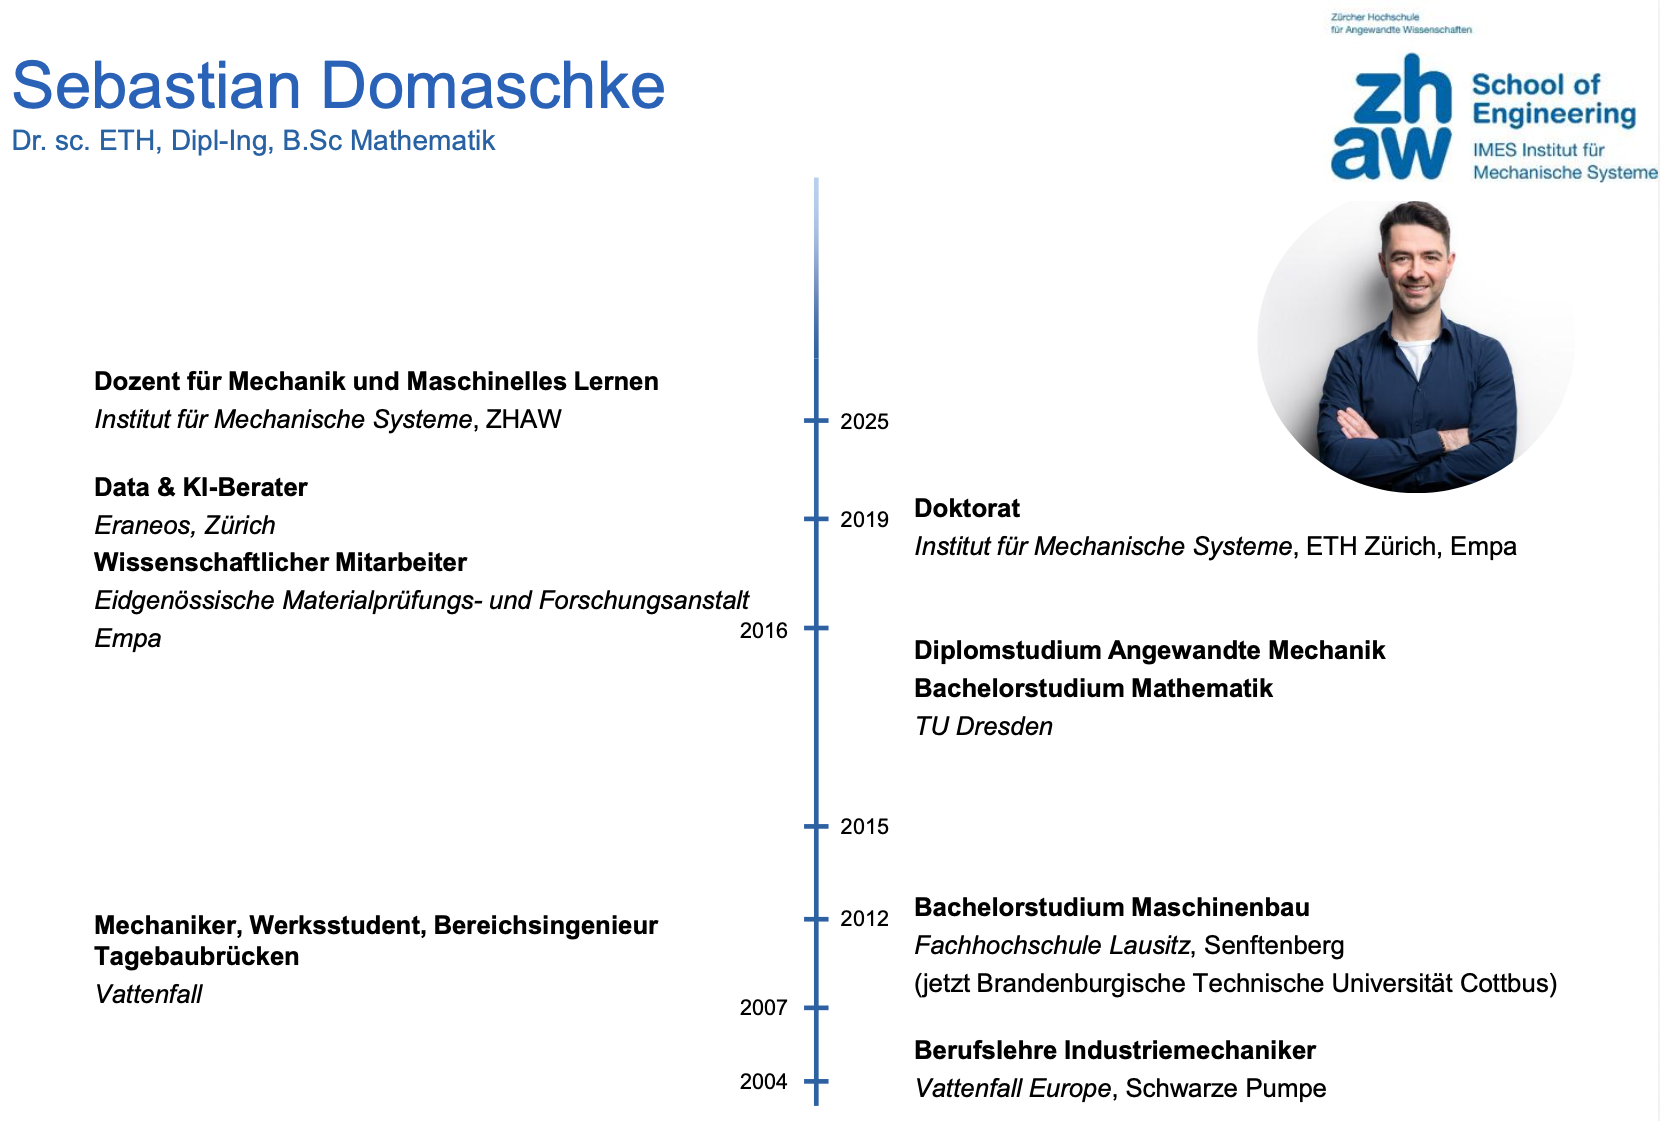
\includegraphics[width=\linewidth,height=0.85\textheight,keepaspectratio]{../Grafiken/Sebastian.png}
\end{frame}

% Was ist FEM?
\begin{frame}{Was ist FEM?}
  \begin{block}{Kurz erklärt}
    FEM ist eine Methode, die physikalische Probleme (z.\,B. Spannungs- oder Temperaturverläufe) auf komplexen Geometrien in ein numerisch lösbares Gleichungssystem $\K\,\uvec=\fvec$ überführt, indem die Geometrie in viele kleine, einfache Elemente zerlegt und die Lösung darin angenähert wird.

    \vspace{0.3em}
    Es ist eines der mächtigsten Hilfsmittel, die Ingenieurinnen und Ingenieure im Studium erlernen.
  \end{block}
  \vspace{0.5em}
  \centering
  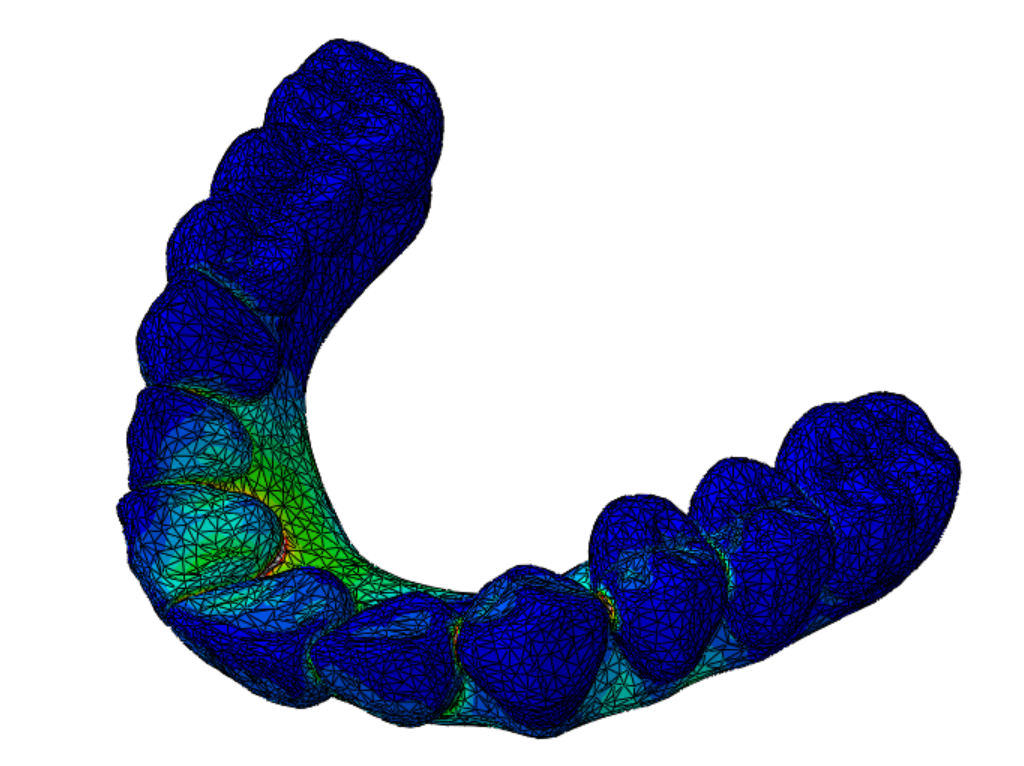
\includegraphics[width=\linewidth,height=0.5\textheight,keepaspectratio]{../Grafiken/Example.png}
\end{frame}

% Wer seid ihr?
\begin{frame}{Wer seid ihr?}
  \Large
  \begin{enumerate}
    \item<1-> \alert<1>{Was ist eure Motivation, FEM zu lernen?}
    \item<2-> \alert<2>{Was glaubt ihr, werden Probleme in diesem Kurs sein?}
    \item<3-> \alert<3>{Was ist euch wichtiger: die Prüfung möglichst gut zu bestehen oder FEM möglichst gut anwenden zu können?}
  \end{enumerate}
\end{frame}

% Agenda
\begin{frame}{Agenda - Übergeordnete Lernziele}
  \begin{columns}[T,onlytextwidth]
    \begin{column}{0.58\textwidth}
      \Large
      \textbf{1. FEM nutzen per Software/Abaqus (nicht prüfungsrelevant.)}

      \vspace{0.9em}
      \textbf{2. Erklärung/Herleitung FEM}\newline
      \textbf{\quad per Matrixsteifigkeitsmethode}

      \vspace{0.9em}
      \textbf{3. Allgemeine Herleitung FEM}\newline
      \textbf{\quad per schwache Form (Galerkin)}
    \end{column}
    \begin{column}{0.42\textwidth}
      \centering
      % TODO: Agenda-Bild einsetzen
      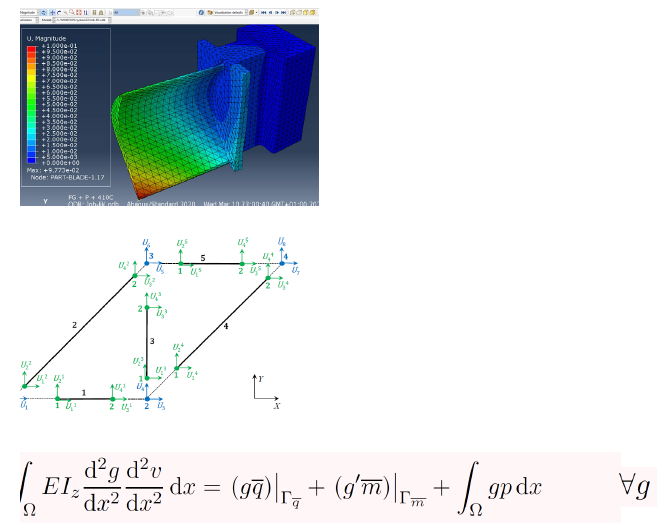
\includegraphics[width=\linewidth,height=0.75\textheight,keepaspectratio]{../Grafiken/Agenda.png}
    \end{column}
  \end{columns}
\end{frame}

% Organisatorisches
\begin{frame}{Organisatorisches}
  \small
  \begin{block}{Modulvereinbarung / Prüfungen}
    \begin{itemize}
      \item Zwischenprüfung: Di., 07.04.2026 (Semesterwoche 8), \textbf{45 Min.}, \textbf{20\%}, Anwesenheitspflicht vor Ort.
      \item Semesterendprüfung (SEP): \textbf{90 Min.}, \textbf{80\%}; Termin wird später im Stundenplan bekanntgegeben.
      \item Kein Bonussystem: Zwischenprüfung wird immer angerechnet.
      \item Kein Nachschreiben der Zwischenprüfung; bei entschuldigtem Fehlen zählt die SEP mit \textbf{100\%}.
      \item Bei Krankheit: ärztliches Attest \textbf{unaufgefordert innert 7 Arbeitstagen} einreichen; sonst Bewertung der versäumten Prüfung mit \textbf{Note 1.0}.
      \item Verboten: Abschreiben, Kommunikation mit Dritten, analoge/digitale Hilfsmittel, Internet.
      \item Erlaubt: nicht-internetfähiger Taschenrechner \& Formelsammlung (max. 2 A4-Seiten: 1 Blatt beidseitig).
      \item Nachteilsausgleich: Nachweis per E-Mail in der \textbf{ersten Vorlesungswoche} an die Dozentin/den Dozenten.
    \end{itemize}
  \end{block}

\end{frame}

% Organisatorisches (Ablageorte)
\begin{frame}{Organisatorisches}
  \small
  \begin{block}{Ablageorte}
    \begin{itemize}
      \item \href{https://teams.microsoft.com/l/team/19\%3AGIHu109EeqabU7ycNk9ORnolyco2HQO7hqafNFYbHHo1\%40thread.tacv2/conversations?groupId=2e4b8463-38a0-41e3-ba6f-93b417edfb12&tenantId=5d1a9f9d-201f-4a10-b983-451cf65cbc1e}{\textbf{Teams (link):}} Ihr solltet alle eingeladen sein; dort findet ihr alles Wichtige zum Kurs.
            \item \href{https://github.com/Boscij/FEM}{\textbf{GitHub(link):}} Begleitend zum Kurs entwickelt ihr dort euren eigenen FEM-Code.
      \item \href{https://moodle.zhaw.ch/course/view.php?id=1979}{\textbf{Moodle allgemein (link):}} Kursübergreifende Ablage mit sehr vielen Infos; für diesen Kurs nicht zwingend nötig, aber schaut gerne einmal rein.

    \end{itemize}
  \end{block}

  \vspace{0.1em}
  \begin{block}{Praktikumsblöcke, TE 223}

Block 1: Dienstag 14:00--15:35 Uhr; Block 2: Dienstag 16:00--17:35 Uhr

  \end{block}
  
  \vspace{0.1em}
  \begin{block}{Literatur}
    \footnotesize
    \begin{itemize}
      \item Fish \& Belytschko: \emph{A First Course in Finite Elements}
      \item Pfrommer, R. (2024). \emph{Die Methode der Finiten Elemente -- Eine Einf\"uhrung}. Lecture Notes, ZHAW.
    \end{itemize}
  \end{block}
\end{frame}

% Warum FEM? (Rückblick Festigkeitslehre)
\begin{frame}{Warum FEM?\;—\;Rückblick Festigkeitslehre}
  \textbf{Frage:} Wonach wurde in den Vorlesungen Festigkeitslehre gesucht?

  \vspace{0.6em}
  \begin{columns}[T,onlytextwidth]
    \begin{column}{0.70\textwidth}
      \centering
      % TODO: Bild 70\% Breite
      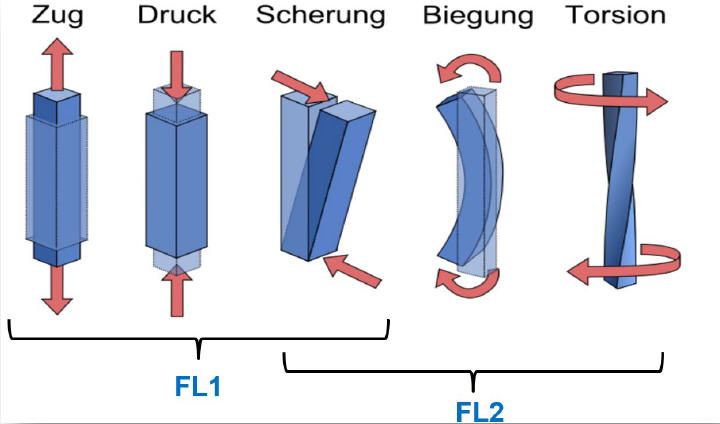
\includegraphics[width=\linewidth,height=0.38\textheight,keepaspectratio]{../Grafiken/FL.png}

      \vspace{0.2em}
      {\footnotesize Einfache Geometrie}
    \end{column}
    \hspace{0.6em}
    \begin{column}{0.28\textwidth}
      \centering
      % TODO: Bild 30\% Breite
      \only<2->{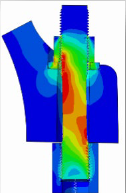
\includegraphics[width=\linewidth,height=0.38\textheight,keepaspectratio]{../Grafiken/KomplexeGeometrie.png}}

      \vspace{0.2em}
      \only<2->{{\footnotesize Komplexe Geometrie (FEM nötig)}}
    \end{column}
  \end{columns}

  \vspace{0.6em}
  \begin{columns}[T,onlytextwidth]
    \begin{column}{0.5\textwidth}
      \centering
      \begin{tikzpicture}[x=1cm,y=1cm]
        % Eingespannte Wand
        \fill[gray!35] (0,0) rectangle (0.35,1.8);
        \foreach \yy in {0.1,0.25,...,1.7} {
          \draw (0,\yy) -- (0.35,\yy+0.15);
        }

        % Kragbalken
        \draw[fill=blue!10,thick] (0.35,0.75) rectangle (5.1,1.05);

        % Einzellast am freien Ende
        \draw[very thick,red,-{Latex[length=3mm]}] (5.1,1.55) -- (5.1,1.05);
        \node[red,above] at (5.1,1.55) {$F$};

        % Koordinatensystem
        \draw[->,thick] (0.4,0.95) -- (1.2,0.95) node[right] {$x$};
        \draw[->,thick] (0.4,0.95) -- (0.4,1.65) node[above] {$y$};

        % L
        \draw[<->] (0.35,0.55) -- (5.1,0.55);
        \node at (2.7,0.42) {$L$};
      \end{tikzpicture}
    \end{column}
    \begin{column}{0.5\textwidth}
      \vfill
      {\scriptsize
      \begin{align*}
        w(x) &= \frac{F x^2}{6 E I}\,(3L-x)\\
        \sigma(x,y) &= \frac{M(x)\,y}{I},\quad M(x)=F(L-x)
      \end{align*}}
    \end{column}
  \end{columns}
\end{frame}

% --- Abschnitt: Motivation ---
\section{Abaqus}

\begin{frame}{Übergeordnetes Lernziel 1}
  \centering
  {\LARGE FEM mittels Softwaretool \textbf{Abaqus}}
\end{frame}

\begin{frame}{Beispiel. Vorführung Analyse Zahnprotese mit Abaqus}
  \centering
  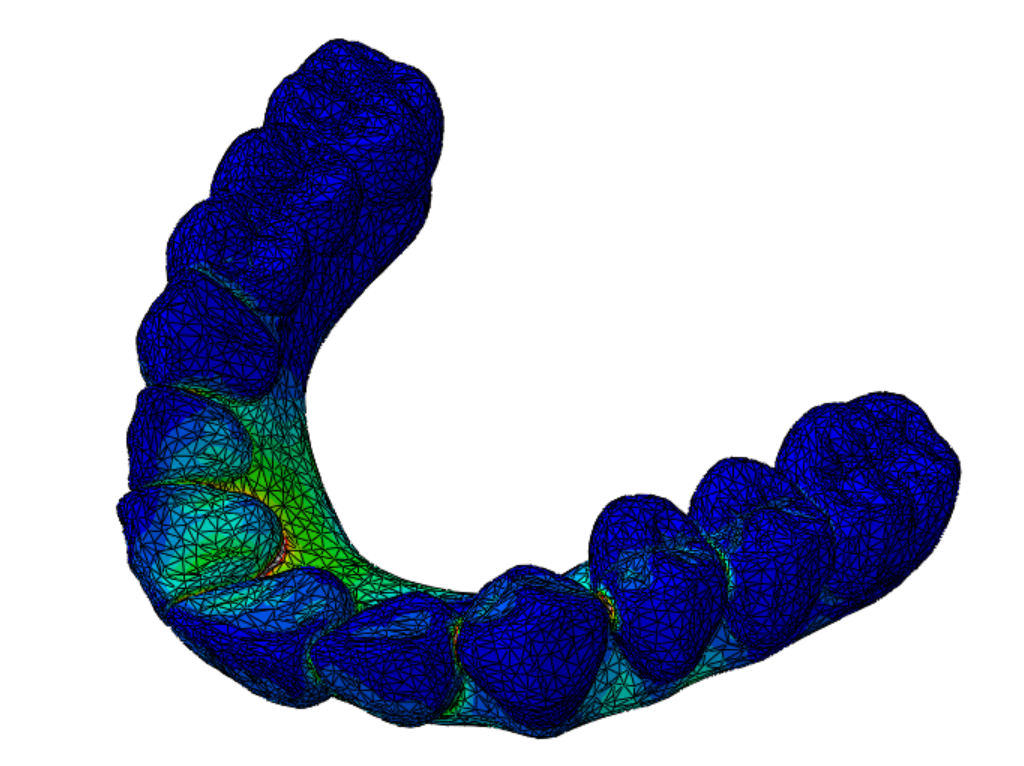
\includegraphics[width=\linewidth,height=0.5\textheight,keepaspectratio]{../Grafiken/Example.png}
\end{frame}

\begin{frame}{Tutorials/Hilfsmittel/Beispiele Abaqus}
  \small
  \begin{itemize}
    \item Das \textbf{Tutorial-Dokument} liegt auf \textbf{Teams}.
    \item Zusätzlich gibt es ein \textbf{Script} mit vielen Inhalten (ebenfalls auf Teams).
    \item Im Praktikum rechnen wir die folgenden Beispiele gemeinsam durch:
  \end{itemize}

  \vspace{0.6em}
  \begin{columns}[T,onlytextwidth]
    \begin{column}{0.33\textwidth}
      \centering
      % TODO: Beispiel 1
      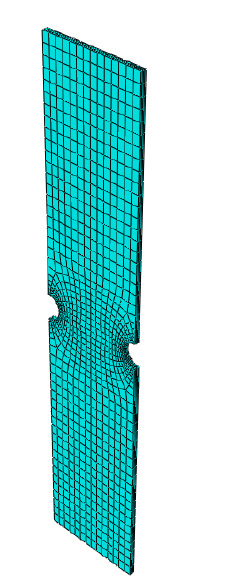
\includegraphics[width=\linewidth,height=0.35\textheight,keepaspectratio]{../Grafiken/Ue1_gekerbtesBlech.png}

      \vspace{0.2em}
      {\footnotesize Gekerbter Blechstreifen unter Zug / Biegung}
    \end{column}
    \begin{column}{0.33\textwidth}
      \centering
      % TODO: Beispiel 2
      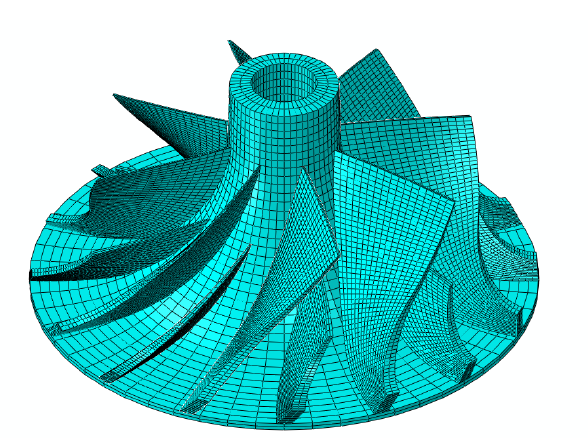
\includegraphics[width=\linewidth,height=0.35\textheight,keepaspectratio]{../Grafiken/Ue2_Radialkompressor.png}

      \vspace{0.2em}
      {\footnotesize Radialkompressor unter Zentrifugallast}
    \end{column}
    \begin{column}{0.33\textwidth}
      \centering
      % TODO: Beispiel 3
      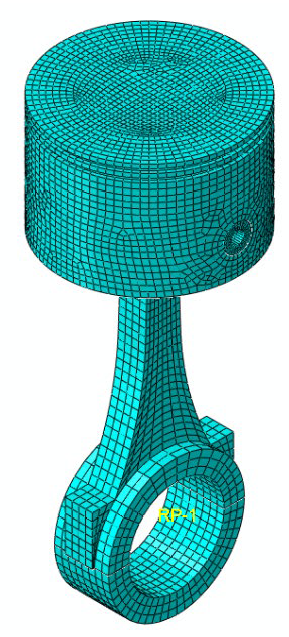
\includegraphics[width=\linewidth,height=0.35\textheight,keepaspectratio]{../Grafiken/Ue3_Kolben.png}

      \vspace{0.2em}
      {\footnotesize Kolben unter Drucklast (Kontakt)}
    \end{column}
  \end{columns}
\end{frame}

\begin{frame}{FEM-Workflow (Übersicht)}
  \centering
  \begin{tikzpicture}[
    x=1cm,y=1cm,
    font=\scriptsize,
    pre/.style={rounded corners=4pt, fill=orange!85!black, text=white, minimum width=6.6cm, minimum height=0.6cm, align=center},
    wfstep/.style={rounded corners=4pt, fill=blue!70!black, text=white, minimum width=6.6cm, minimum height=0.6cm, align=center},
    post/.style={rounded corners=4pt, fill=red!80!black, text=white, minimum width=6.6cm, minimum height=0.6cm, align=center},
    legend/.style={rounded corners=3pt, text=white, minimum width=3.1cm, text width=3.1cm, minimum height=0.45cm, align=center},
    bigarrow/.style={-Latex, line width=2.2pt}
  ]
    % Legende (rechts oben, ohne Überlappung)
    \node[legend, fill=orange!85!black, anchor=north west] at (4.05,2.55) {Preprocessing};
    \node[legend, fill=blue!70!black,   anchor=north west] at (4.05,2.00) {Core};
    \node[legend, fill=red!80!black,    anchor=north west] at (4.05,1.45) {Postprocessing};

    % Schritte (ohne einzelne Pfeile)
    \node[pre]    (p1) at (0,2.0) {Problem definieren (Geometrie, Material, Lasten)};
    \node[pre]    (p2) at (0,1.1) {Diskretisieren (Netz/Elemente)};
    \node[pre]    (p3) at (0,0.2) {Randbedingungen setzen (Lager, Kontakte)};
    \node[wfstep] (p4) at (0,-0.7) {Elementsteifigkeitsmatrix $\mathbf{k}^e$ berechnen};
    \node[wfstep] (p5) at (0,-1.6) {Global assemblieren $\mathbf{K}$ und $\mathbf{f}$};
    \node[wfstep] (p6) at (0,-2.5) {Gleichungssystem lösen $\mathbf{K}\,\mathbf{u}=\mathbf{f}$};

    % Ein großer Pfeil rechts (oben nach unten)
    \draw[bigarrow] (3.8,2.25) -- (3.8,-2.95);

    % Unten: Post/Valid (ohne Pfeile)
    \node[post, minimum width=4.0cm] (post) at (-2.1,-3.4) {Post-Processing};
    \node[post, minimum width=4.0cm] (val)  at ( 2.1,-3.4) {Validierung};

    % Bounding box
    \path (-4.6,2.6) rectangle (4.6,-3.8);
  \end{tikzpicture}
\end{frame}

\begin{frame}{Übergeordnetes Lernziel 2}
  \centering
  \begin{minipage}{0.9\linewidth}
    \centering
    {\LARGE  Herleitung / Erklärung FEM\\[0.6em]}
    {\Large bestehend aus 1D-Elementen (Federn, Stäben, Balken)\\[0.4em]}
    {\Large mittels \textbf{Matrixsteifigkeitsmethode}}
  \end{minipage}
\end{frame}

% Motivation
\begin{frame}{Motivation}
  \begin{columns}[T,onlytextwidth]
    \begin{column}{0.49\textwidth}
      \centering
      % TODO: Bild 1 ersetzen
      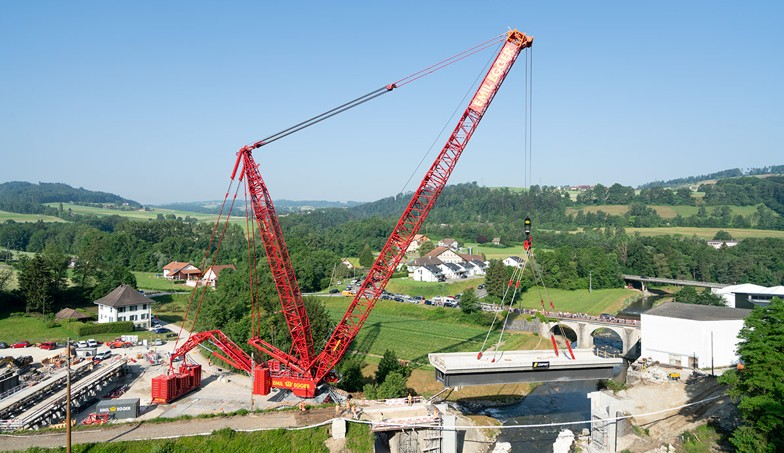
\includegraphics[width=\linewidth,height=0.62\textheight,keepaspectratio]{../Grafiken/Liebherr.jpg}

      \vspace{0.2em}
      {\footnotesize Liebherr LR 11000}
    \end{column}
    \hspace{0.02\textwidth}
    \begin{column}{0.49\textwidth}
      \centering
      % TODO: Bild 2 ersetzen
      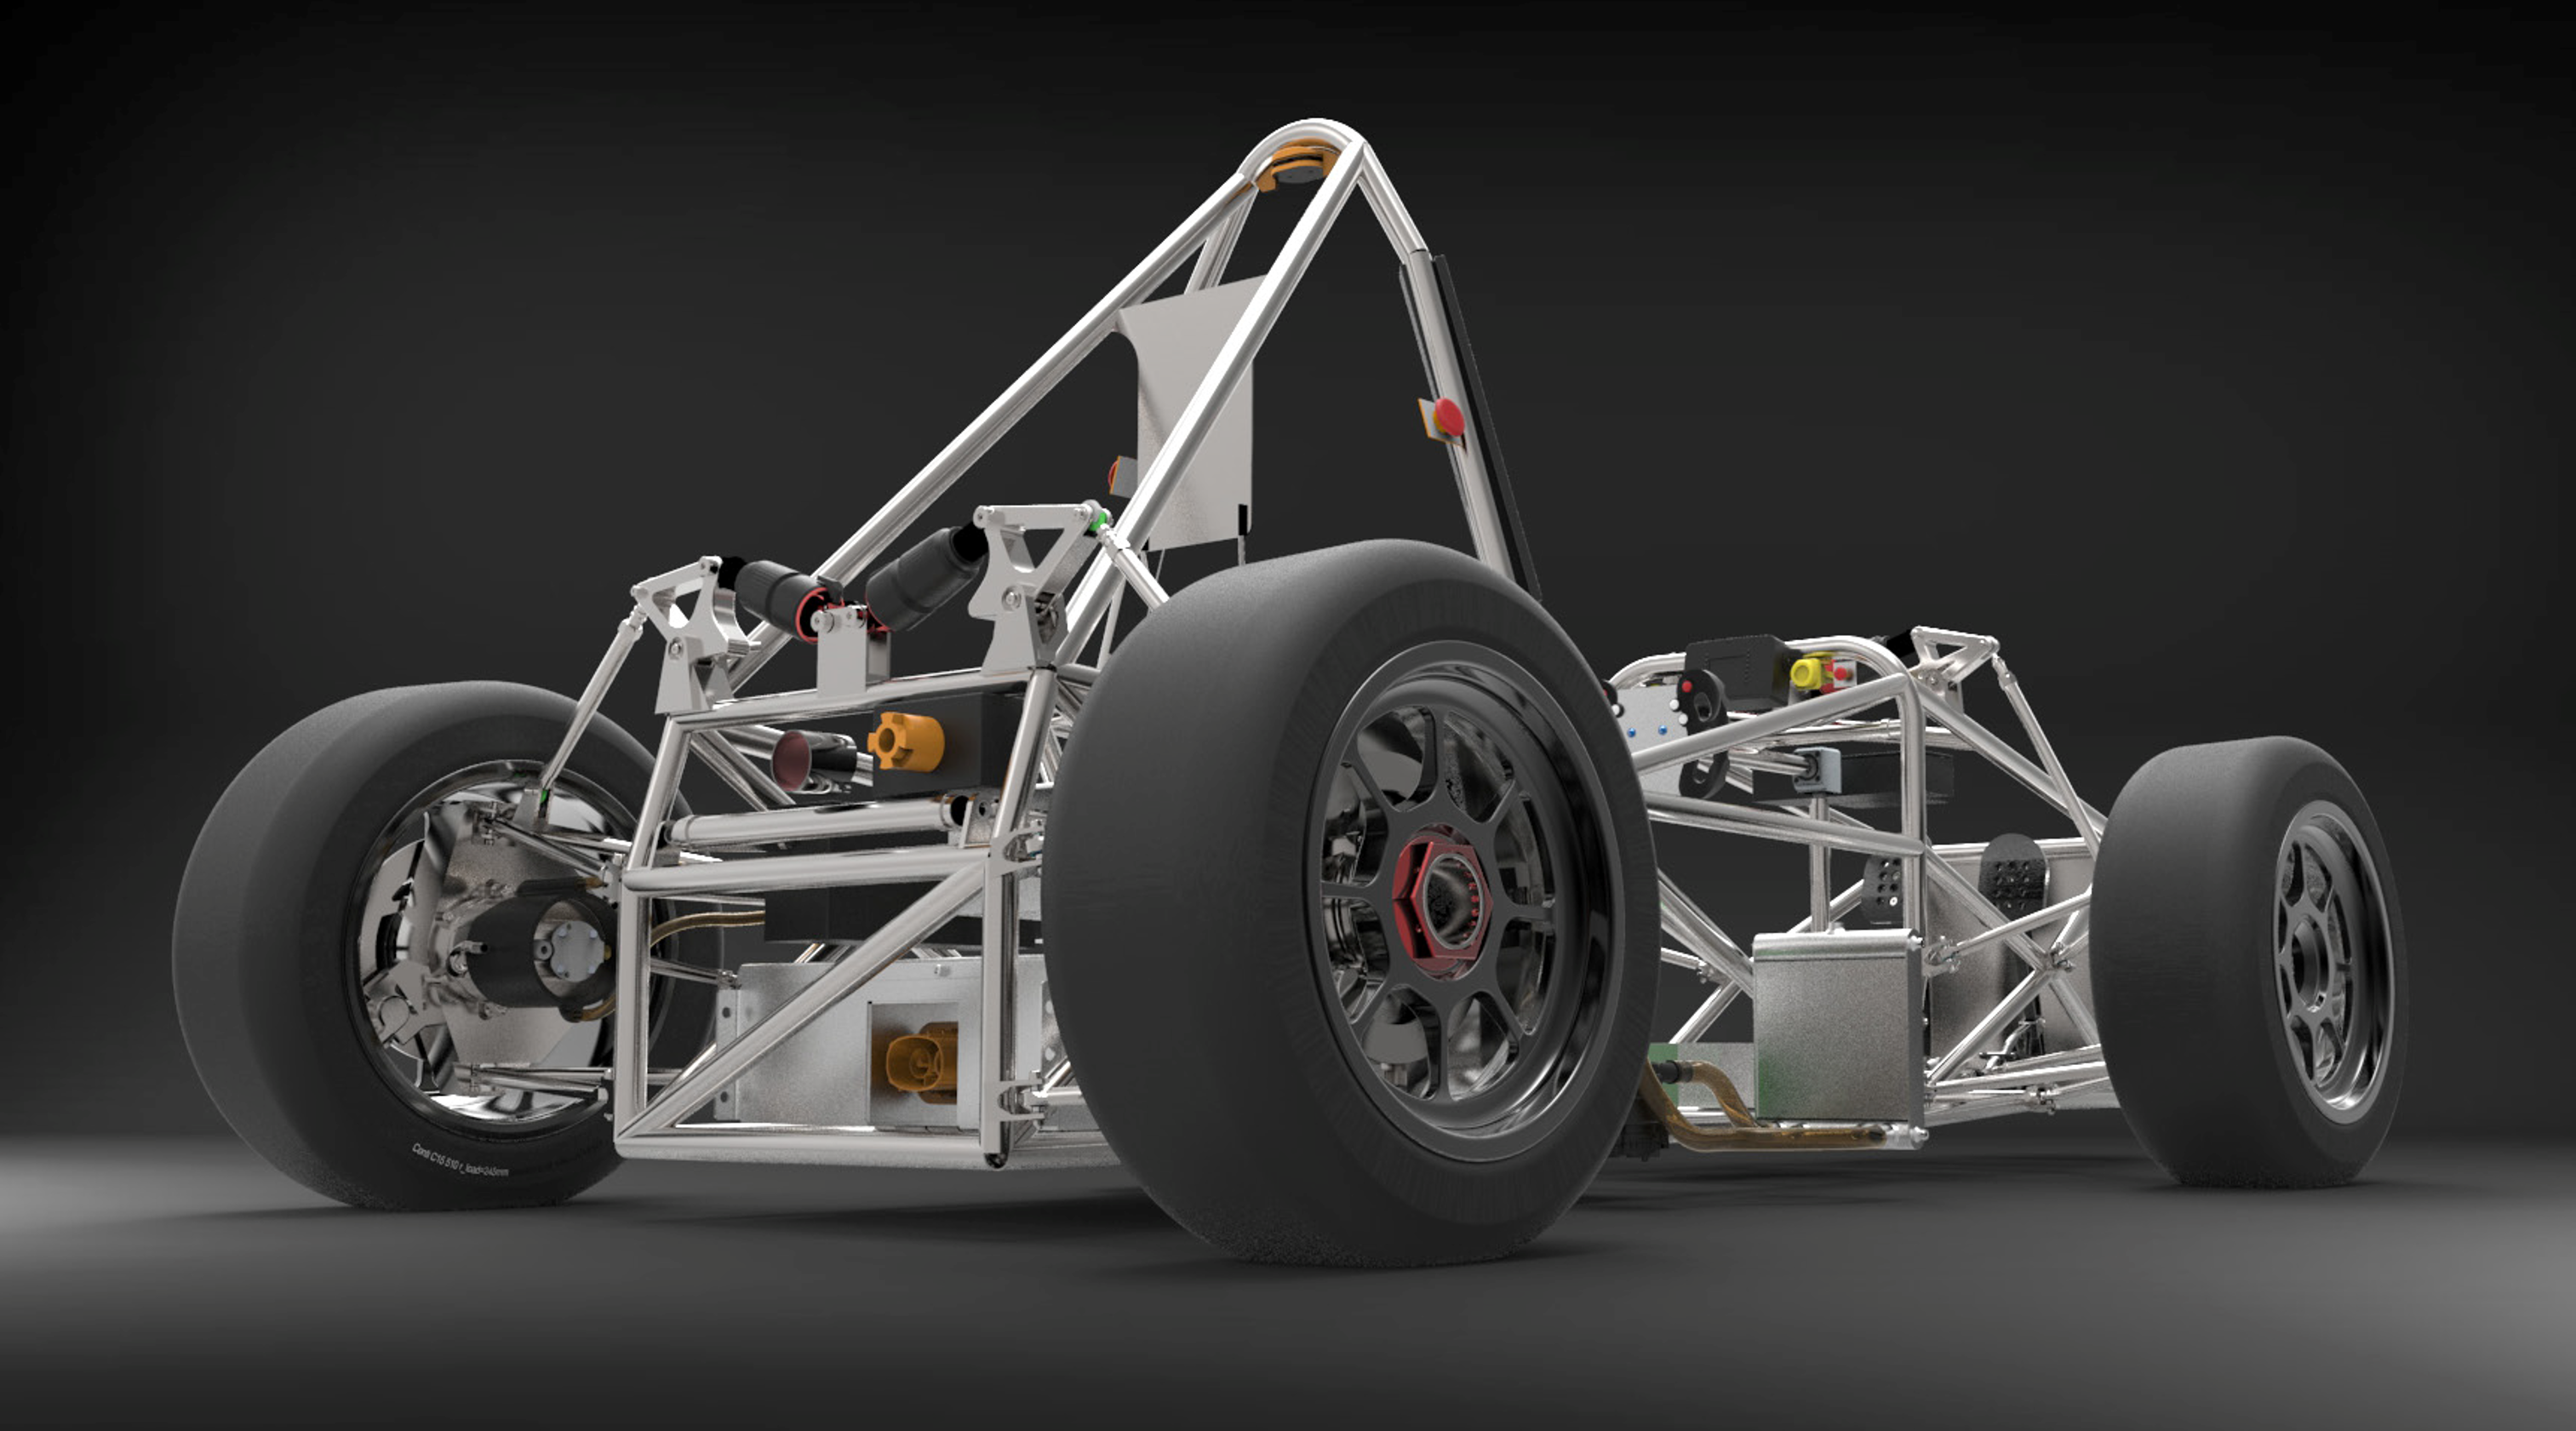
\includegraphics[width=\linewidth,height=0.62\textheight,keepaspectratio]{../Grafiken/FormulaStudent.png}

      \vspace{0.2em}
      {\footnotesize Formula Student}
    \end{column}
  \end{columns}

  \vspace{0.3em}
  \footnotesize
  \footnote{Quellenlinks: (1) \href{https://www.liebherr.com/de/che/produkte/mobil-und-raupenkrane/kundenmagazin/alles-ueber-krane/v-frame.html
\includegraphics[width=0.5\textwidth]{image.png}}{www.liebherr.com}, (2) \href{https://www.inneo.de/files/content/Download/Referenzen/bern-formula-student-106249-20170504.pdf
\includegraphics[width=0.5\textwidth]{image_2.png}}{www.inneo.de}.}
\end{frame}



\begin{frame}{Literatur / Ressourcen}
  \begin{itemize}
    \item Fish \& Belytschko: \emph{A First Course in Finite Elements}
    \item Pfrommer, R. (2024). \emph{Die Methode der Finiten Elemente -- Eine Einf\"uhrung}. Lecture Notes, ZHAW.
  \end{itemize}
\end{frame}




\end{document}